\documentclass[twoside]{book}

% Packages required by doxygen
\usepackage{fixltx2e}
\usepackage{calc}
\usepackage{doxygen}
\usepackage[export]{adjustbox} % also loads graphicx
\usepackage{graphicx}
\usepackage[utf8]{inputenc}
\usepackage{makeidx}
\usepackage{multicol}
\usepackage{multirow}
\PassOptionsToPackage{warn}{textcomp}
\usepackage{textcomp}
\usepackage[nointegrals]{wasysym}
\usepackage[table]{xcolor}

% Font selection
\usepackage[T1]{fontenc}
\usepackage[scaled=.90]{helvet}
\usepackage{courier}
\usepackage{amssymb}
\usepackage{sectsty}
\renewcommand{\familydefault}{\sfdefault}
\allsectionsfont{%
  \fontseries{bc}\selectfont%
  \color{darkgray}%
}
\renewcommand{\DoxyLabelFont}{%
  \fontseries{bc}\selectfont%
  \color{darkgray}%
}
\newcommand{\+}{\discretionary{\mbox{\scriptsize$\hookleftarrow$}}{}{}}

% Page & text layout
\usepackage{geometry}
\geometry{%
  a4paper,%
  top=2.5cm,%
  bottom=2.5cm,%
  left=2.5cm,%
  right=2.5cm%
}
\tolerance=750
\hfuzz=15pt
\hbadness=750
\setlength{\emergencystretch}{15pt}
\setlength{\parindent}{0cm}
\setlength{\parskip}{3ex plus 2ex minus 2ex}
\makeatletter
\renewcommand{\paragraph}{%
  \@startsection{paragraph}{4}{0ex}{-1.0ex}{1.0ex}{%
    \normalfont\normalsize\bfseries\SS@parafont%
  }%
}
\renewcommand{\subparagraph}{%
  \@startsection{subparagraph}{5}{0ex}{-1.0ex}{1.0ex}{%
    \normalfont\normalsize\bfseries\SS@subparafont%
  }%
}
\makeatother

% Headers & footers
\usepackage{fancyhdr}
\pagestyle{fancyplain}
\fancyhead[LE]{\fancyplain{}{\bfseries\thepage}}
\fancyhead[CE]{\fancyplain{}{}}
\fancyhead[RE]{\fancyplain{}{\bfseries\leftmark}}
\fancyhead[LO]{\fancyplain{}{\bfseries\rightmark}}
\fancyhead[CO]{\fancyplain{}{}}
\fancyhead[RO]{\fancyplain{}{\bfseries\thepage}}
\fancyfoot[LE]{\fancyplain{}{}}
\fancyfoot[CE]{\fancyplain{}{}}
\fancyfoot[RE]{\fancyplain{}{\bfseries\scriptsize Generated by Doxygen }}
\fancyfoot[LO]{\fancyplain{}{\bfseries\scriptsize Generated by Doxygen }}
\fancyfoot[CO]{\fancyplain{}{}}
\fancyfoot[RO]{\fancyplain{}{}}
\renewcommand{\footrulewidth}{0.4pt}
\renewcommand{\chaptermark}[1]{%
  \markboth{#1}{}%
}
\renewcommand{\sectionmark}[1]{%
  \markright{\thesection\ #1}%
}

% Indices & bibliography
\usepackage{natbib}
\usepackage[titles]{tocloft}
\setcounter{tocdepth}{3}
\setcounter{secnumdepth}{5}
\makeindex

% Hyperlinks (required, but should be loaded last)
\usepackage{ifpdf}
\ifpdf
  \usepackage[pdftex,pagebackref=true]{hyperref}
\else
  \usepackage[ps2pdf,pagebackref=true]{hyperref}
\fi
\hypersetup{%
  colorlinks=true,%
  linkcolor=blue,%
  citecolor=blue,%
  unicode%
}

% Custom commands
\newcommand{\clearemptydoublepage}{%
  \newpage{\pagestyle{empty}\cleardoublepage}%
}

\usepackage{caption}
\captionsetup{labelsep=space,justification=centering,font={bf},singlelinecheck=off,skip=4pt,position=top}

%===== C O N T E N T S =====

\begin{document}

% Titlepage & ToC
\hypersetup{pageanchor=false,
             bookmarksnumbered=true,
             pdfencoding=unicode
            }
\pagenumbering{alph}
\begin{titlepage}
\vspace*{7cm}
\begin{center}%
{\Large Couleuvre-\/\+X\+OR }\\
\vspace*{1cm}
{\large Generated by Doxygen 1.8.14}\\
\end{center}
\end{titlepage}
\clearemptydoublepage
\pagenumbering{roman}
\tableofcontents
\clearemptydoublepage
\pagenumbering{arabic}
\hypersetup{pageanchor=true}

%--- Begin generated contents ---
\chapter{Couleuvre-\/\+X\+OR}
\label{md_README}
\Hypertarget{md_README}
Projet de réseau modélisant le X\+OR logique, en C++ 
\chapter{Hierarchical Index}
\section{Class Hierarchy}
This inheritance list is sorted roughly, but not completely, alphabetically\+:\begin{DoxyCompactList}
\item \contentsline{section}{Application}{\pageref{classApplication}}{}
\item \contentsline{section}{csvfile}{\pageref{classcsvfile}}{}
\item \contentsline{section}{Statistics\+:\+:Data}{\pageref{structStatistics_1_1Data}}{}
\item \contentsline{section}{Data\+Collector}{\pageref{classDataCollector}}{}
\item \contentsline{section}{Data\+Set}{\pageref{classDataSet}}{}
\item \contentsline{section}{Stats\+:\+:Error\+Collector}{\pageref{classStats_1_1ErrorCollector}}{}
\item \contentsline{section}{Functions}{\pageref{structFunctions}}{}
\item list\begin{DoxyCompactList}
\item \contentsline{section}{Neural\+Network}{\pageref{classNeuralNetwork}}{}
\end{DoxyCompactList}
\item \contentsline{section}{Neuron\+Layer}{\pageref{classNeuronLayer}}{}
\item \contentsline{section}{Stats\+:\+:Error\+Collector\+:\+:Statistic\+Data}{\pageref{structStats_1_1ErrorCollector_1_1StatisticData}}{}
\item \contentsline{section}{Statistics}{\pageref{classStatistics}}{}
\item \contentsline{section}{Stats\+:\+:Stats\+Collector}{\pageref{classStats_1_1StatsCollector}}{}
\item \contentsline{section}{Teacher}{\pageref{classTeacher}}{}
\end{DoxyCompactList}

\chapter{Class Index}
\section{Class List}
Here are the classes, structs, unions and interfaces with brief descriptions\+:\begin{DoxyCompactList}
\item\contentsline{section}{\hyperlink{classApplication}{Application} \\*Classe destinée à gérer l\textquotesingle{}ensemble d\textquotesingle{}un projet }{\pageref{classApplication}}{}
\item\contentsline{section}{\hyperlink{classcsvfile}{csvfile} }{\pageref{classcsvfile}}{}
\item\contentsline{section}{\hyperlink{structStatistics_1_1Data}{Statistics\+::\+Data} \\*Structure contenant les mesures d\textquotesingle{}un jeu de donnée }{\pageref{structStatistics_1_1Data}}{}
\item\contentsline{section}{\hyperlink{classDataCollector}{Data\+Collector} }{\pageref{classDataCollector}}{}
\item\contentsline{section}{\hyperlink{classDataSet}{Data\+Set} }{\pageref{classDataSet}}{}
\item\contentsline{section}{\hyperlink{structFunctions}{Functions} }{\pageref{structFunctions}}{}
\item\contentsline{section}{\hyperlink{classNeuralNetwork}{Neural\+Network} }{\pageref{classNeuralNetwork}}{}
\item\contentsline{section}{\hyperlink{classNeuronLayer}{Neuron\+Layer} \\*Classe modélisant une couche de neurones }{\pageref{classNeuronLayer}}{}
\item\contentsline{section}{\hyperlink{classStatistics}{Statistics} }{\pageref{classStatistics}}{}
\item\contentsline{section}{\hyperlink{classTeacher}{Teacher} }{\pageref{classTeacher}}{}
\end{DoxyCompactList}

\chapter{Class Documentation}
\hypertarget{structFunctions}{}\section{Functions Struct Reference}
\label{structFunctions}\index{Functions@{Functions}}


{\ttfamily \#include $<$functions.\+hpp$>$}



Collaboration diagram for Functions\+:
\nopagebreak
\begin{figure}[H]
\begin{center}
\leavevmode
\includegraphics[width=156pt]{structFunctions__coll__graph}
\end{center}
\end{figure}
\subsection*{Public Types}
\begin{DoxyCompactItemize}
\item 
using \hyperlink{structFunctions_ad25362ffa52b2f7933431190546593ac}{Activation\+Fun} = std\+::function$<$ float(float)$>$
\item 
using \hyperlink{structFunctions_a834bc4170f1caa8c77272ecf51dbae5c}{Error\+Fun} = std\+::function$<$ float(Eigen\+::\+Vector\+Xf, Eigen\+::\+Vector\+Xf)$>$
\end{DoxyCompactItemize}
\subsection*{Static Public Member Functions}
\begin{DoxyCompactItemize}
\item 
static \hyperlink{structFunctions_ad25362ffa52b2f7933431190546593ac}{Activation\+Fun} \hyperlink{structFunctions_a773de9cd59f7ccc3e2fe9822f0536ae4}{sigmoid} (float lambda)
\item 
static \hyperlink{structFunctions_ad25362ffa52b2f7933431190546593ac}{Activation\+Fun} \hyperlink{structFunctions_a683c495693f3e2a5ec55e30edaccfd2d}{heavyside} (float gap\+Abscissa)
\item 
static \hyperlink{structFunctions_ad25362ffa52b2f7933431190546593ac}{Activation\+Fun} \hyperlink{structFunctions_a0aac84382fccbc38cacccd566434d4a8}{hyper\+Tan} ()
\item 
static \hyperlink{structFunctions_a834bc4170f1caa8c77272ecf51dbae5c}{Error\+Fun} \hyperlink{structFunctions_a00bac40f42bb6c47d25c0cd238c4275a}{l2\+Norm} ()
\end{DoxyCompactItemize}


\subsection{Member Typedef Documentation}
\mbox{\Hypertarget{structFunctions_ad25362ffa52b2f7933431190546593ac}\label{structFunctions_ad25362ffa52b2f7933431190546593ac}} 
\index{Functions@{Functions}!Activation\+Fun@{Activation\+Fun}}
\index{Activation\+Fun@{Activation\+Fun}!Functions@{Functions}}
\subsubsection{\texorpdfstring{Activation\+Fun}{ActivationFun}}
{\footnotesize\ttfamily using \hyperlink{structFunctions_ad25362ffa52b2f7933431190546593ac}{Functions\+::\+Activation\+Fun} =  std\+::function$<$float(float)$>$}

\mbox{\Hypertarget{structFunctions_a834bc4170f1caa8c77272ecf51dbae5c}\label{structFunctions_a834bc4170f1caa8c77272ecf51dbae5c}} 
\index{Functions@{Functions}!Error\+Fun@{Error\+Fun}}
\index{Error\+Fun@{Error\+Fun}!Functions@{Functions}}
\subsubsection{\texorpdfstring{Error\+Fun}{ErrorFun}}
{\footnotesize\ttfamily using \hyperlink{structFunctions_a834bc4170f1caa8c77272ecf51dbae5c}{Functions\+::\+Error\+Fun} =  std\+::function$<$float(Eigen\+::\+Vector\+Xf, Eigen\+::\+Vector\+Xf)$>$}



\subsection{Member Function Documentation}
\mbox{\Hypertarget{structFunctions_a683c495693f3e2a5ec55e30edaccfd2d}\label{structFunctions_a683c495693f3e2a5ec55e30edaccfd2d}} 
\index{Functions@{Functions}!heavyside@{heavyside}}
\index{heavyside@{heavyside}!Functions@{Functions}}
\subsubsection{\texorpdfstring{heavyside()}{heavyside()}}
{\footnotesize\ttfamily \hyperlink{structFunctions_ad25362ffa52b2f7933431190546593ac}{Functions\+::\+Activation\+Fun} Functions\+::heavyside (\begin{DoxyParamCaption}\item[{float}]{gap\+Abscissa }\end{DoxyParamCaption})\hspace{0.3cm}{\ttfamily [static]}}

\mbox{\Hypertarget{structFunctions_a0aac84382fccbc38cacccd566434d4a8}\label{structFunctions_a0aac84382fccbc38cacccd566434d4a8}} 
\index{Functions@{Functions}!hyper\+Tan@{hyper\+Tan}}
\index{hyper\+Tan@{hyper\+Tan}!Functions@{Functions}}
\subsubsection{\texorpdfstring{hyper\+Tan()}{hyperTan()}}
{\footnotesize\ttfamily \hyperlink{structFunctions_ad25362ffa52b2f7933431190546593ac}{Functions\+::\+Activation\+Fun} Functions\+::hyper\+Tan (\begin{DoxyParamCaption}{ }\end{DoxyParamCaption})\hspace{0.3cm}{\ttfamily [static]}}

\mbox{\Hypertarget{structFunctions_a00bac40f42bb6c47d25c0cd238c4275a}\label{structFunctions_a00bac40f42bb6c47d25c0cd238c4275a}} 
\index{Functions@{Functions}!l2\+Norm@{l2\+Norm}}
\index{l2\+Norm@{l2\+Norm}!Functions@{Functions}}
\subsubsection{\texorpdfstring{l2\+Norm()}{l2Norm()}}
{\footnotesize\ttfamily \hyperlink{structFunctions_a834bc4170f1caa8c77272ecf51dbae5c}{Functions\+::\+Error\+Fun} Functions\+::l2\+Norm (\begin{DoxyParamCaption}{ }\end{DoxyParamCaption})\hspace{0.3cm}{\ttfamily [static]}}

\mbox{\Hypertarget{structFunctions_a773de9cd59f7ccc3e2fe9822f0536ae4}\label{structFunctions_a773de9cd59f7ccc3e2fe9822f0536ae4}} 
\index{Functions@{Functions}!sigmoid@{sigmoid}}
\index{sigmoid@{sigmoid}!Functions@{Functions}}
\subsubsection{\texorpdfstring{sigmoid()}{sigmoid()}}
{\footnotesize\ttfamily \hyperlink{structFunctions_ad25362ffa52b2f7933431190546593ac}{Functions\+::\+Activation\+Fun} Functions\+::sigmoid (\begin{DoxyParamCaption}\item[{float}]{lambda }\end{DoxyParamCaption})\hspace{0.3cm}{\ttfamily [static]}}



The documentation for this struct was generated from the following files\+:\begin{DoxyCompactItemize}
\item 
headers/\hyperlink{functions_8hpp}{functions.\+hpp}\item 
sources/\hyperlink{functions_8cpp}{functions.\+cpp}\end{DoxyCompactItemize}

\hypertarget{classNeuralNetwork}{}\section{Neural\+Network Class Reference}
\label{classNeuralNetwork}\index{Neural\+Network@{Neural\+Network}}
Inheritance diagram for Neural\+Network\+:\begin{figure}[H]
\begin{center}
\leavevmode
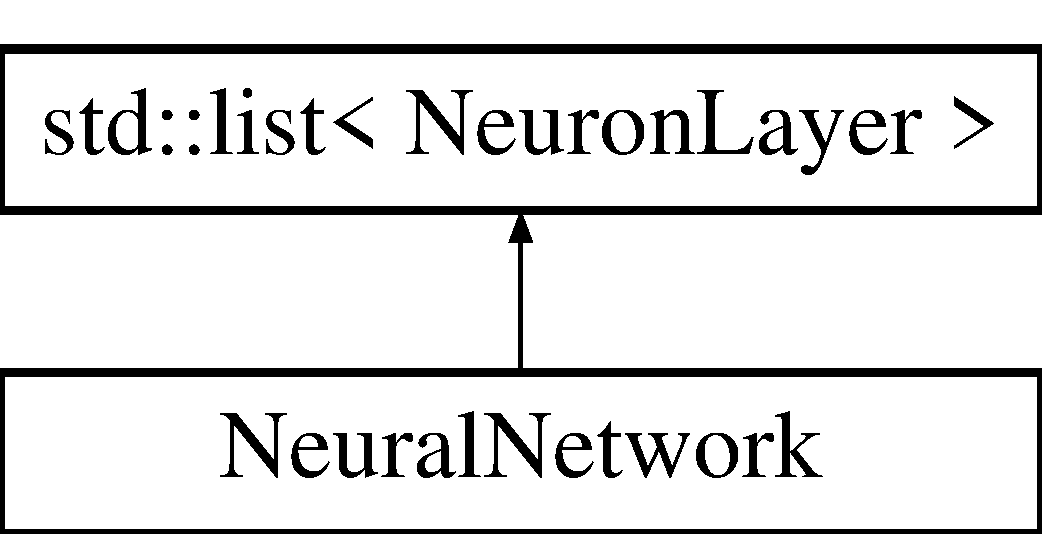
\includegraphics[height=2.000000cm]{classNeuralNetwork}
\end{center}
\end{figure}
\subsection*{Public Types}
\begin{DoxyCompactItemize}
\item 
\mbox{\Hypertarget{classNeuralNetwork_a31de381df65f261fd0f38e0559995d1a}\label{classNeuralNetwork_a31de381df65f261fd0f38e0559995d1a}} 
using {\bfseries Ptr} = std\+::shared\+\_\+ptr$<$ \hyperlink{classNeuralNetwork}{Neural\+Network} $>$
\end{DoxyCompactItemize}
\subsection*{Public Member Functions}
\begin{DoxyCompactItemize}
\item 
\mbox{\Hypertarget{classNeuralNetwork_accce4a7728e89a009a9d4ca1758c9b9d}\label{classNeuralNetwork_accce4a7728e89a009a9d4ca1758c9b9d}} 
\hyperlink{classNeuralNetwork_accce4a7728e89a009a9d4ca1758c9b9d}{Neural\+Network} ()
\begin{DoxyCompactList}\small\item\em Constructeur permettant d\textquotesingle{}initialiser une réseau neuronal vide. \end{DoxyCompactList}\item 
\hyperlink{classNeuralNetwork_a85cd20f411e96dfd28954fcda39badb7}{Neural\+Network} (std\+::vector$<$ unsigned int $>$ layer\+Sizes, std\+::vector$<$ Functions\+::\+Activation\+Fun $>$ activation\+Funs)
\begin{DoxyCompactList}\small\item\em Constructeur permettant d\textquotesingle{}initialiser un réseau neuronal avec choix des fonctions d\textquotesingle{}activation. \end{DoxyCompactList}\item 
\hyperlink{classNeuralNetwork_ab4015471a72a3d00b6bcabf156526f7b}{Neural\+Network} (std\+::vector$<$ unsigned int $>$ layer\+Sizes)
\begin{DoxyCompactList}\small\item\em Constructeur permettant d\textquotesingle{}initialiser un réseau neuronal avec la fonction par défaut. \end{DoxyCompactList}\item 
{\footnotesize template$<$typename Container $>$ }\\\hyperlink{classNeuralNetwork_a7943bb4e9cb96aae048b236d4f1dd979}{Neural\+Network} (Container layer\+List)
\begin{DoxyCompactList}\small\item\em Constructeur permettant d\textquotesingle{}initialiser le réseau neuronal avec un conteneur (vector, list...) de neuron\+Layer. \end{DoxyCompactList}\item 
\mbox{\Hypertarget{classNeuralNetwork_a98cab3b3726fbf06dca316068c29c783}\label{classNeuralNetwork_a98cab3b3726fbf06dca316068c29c783}} 
Eigen\+::\+Vector\+Xf {\bfseries process} (Eigen\+::\+Vector\+Xf input)
\end{DoxyCompactItemize}
\subsection*{Friends}
\begin{DoxyCompactItemize}
\item 
std\+::ostream \& \hyperlink{classNeuralNetwork_a0ecebf9a494437efb917804ed271e13f}{operator$<$$<$} (std\+::ostream \&flux, \hyperlink{classNeuralNetwork}{Neural\+Network} network)
\begin{DoxyCompactList}\small\item\em Fonction utilitaire permettant d\textquotesingle{}afficher le réseau de neurones. \end{DoxyCompactList}\end{DoxyCompactItemize}


\subsection{Constructor \& Destructor Documentation}
\mbox{\Hypertarget{classNeuralNetwork_a85cd20f411e96dfd28954fcda39badb7}\label{classNeuralNetwork_a85cd20f411e96dfd28954fcda39badb7}} 
\index{Neural\+Network@{Neural\+Network}!Neural\+Network@{Neural\+Network}}
\index{Neural\+Network@{Neural\+Network}!Neural\+Network@{Neural\+Network}}
\subsubsection{\texorpdfstring{Neural\+Network()}{NeuralNetwork()}\hspace{0.1cm}{\footnotesize\ttfamily [1/3]}}
{\footnotesize\ttfamily Neural\+Network\+::\+Neural\+Network (\begin{DoxyParamCaption}\item[{std\+::vector$<$ unsigned int $>$}]{layer\+Sizes,  }\item[{std\+::vector$<$ Functions\+::\+Activation\+Fun $>$}]{activation\+Funs }\end{DoxyParamCaption})}



Constructeur permettant d\textquotesingle{}initialiser un réseau neuronal avec choix des fonctions d\textquotesingle{}activation. 

Constructeur permettant l\textquotesingle{}initialisation d\textquotesingle{}un réseau à n couches à partir des (n+1) tailles d\textquotesingle{}input/output (la sortie d\textquotesingle{}une couche est l\textquotesingle{}entrée de la suivante), avec choix des fonctions d\textquotesingle{}activation 
\begin{DoxyParams}{Parameters}
{\em layer\+Sizes} & les tailles des vecteurs d\textquotesingle{}entrées/sorties \\
\hline
{\em activation\+Funs} & le vector contenant les fonctions d\textquotesingle{}activation de chaque couche \\
\hline
\end{DoxyParams}
\mbox{\Hypertarget{classNeuralNetwork_ab4015471a72a3d00b6bcabf156526f7b}\label{classNeuralNetwork_ab4015471a72a3d00b6bcabf156526f7b}} 
\index{Neural\+Network@{Neural\+Network}!Neural\+Network@{Neural\+Network}}
\index{Neural\+Network@{Neural\+Network}!Neural\+Network@{Neural\+Network}}
\subsubsection{\texorpdfstring{Neural\+Network()}{NeuralNetwork()}\hspace{0.1cm}{\footnotesize\ttfamily [2/3]}}
{\footnotesize\ttfamily Neural\+Network\+::\+Neural\+Network (\begin{DoxyParamCaption}\item[{std\+::vector$<$ unsigned int $>$}]{layer\+Sizes }\end{DoxyParamCaption})}



Constructeur permettant d\textquotesingle{}initialiser un réseau neuronal avec la fonction par défaut. 

Constructeur permettant l\textquotesingle{}initialisation d\textquotesingle{}un réseau à n couches à partir des (n+1) tailles d\textquotesingle{}input/output (la sortie d\textquotesingle{}une couche est l\textquotesingle{}entrée de la suivante). La fonction d\textquotesingle{}activation choisie est la fonction d\textquotesingle{}activation par défaut 
\begin{DoxyParams}{Parameters}
{\em layer\+Sizes} & les tailles des vecteurs d\textquotesingle{}entrées/sorties \\
\hline
\end{DoxyParams}
\mbox{\Hypertarget{classNeuralNetwork_a7943bb4e9cb96aae048b236d4f1dd979}\label{classNeuralNetwork_a7943bb4e9cb96aae048b236d4f1dd979}} 
\index{Neural\+Network@{Neural\+Network}!Neural\+Network@{Neural\+Network}}
\index{Neural\+Network@{Neural\+Network}!Neural\+Network@{Neural\+Network}}
\subsubsection{\texorpdfstring{Neural\+Network()}{NeuralNetwork()}\hspace{0.1cm}{\footnotesize\ttfamily [3/3]}}
{\footnotesize\ttfamily template$<$typename Container $>$ \\
Neural\+Network\+::\+Neural\+Network (\begin{DoxyParamCaption}\item[{Container}]{layer\+List }\end{DoxyParamCaption})}



Constructeur permettant d\textquotesingle{}initialiser le réseau neuronal avec un conteneur (vector, list...) de neuron\+Layer. 


\begin{DoxyParams}{Parameters}
{\em layer\+List} & la liste des couches de neurones \\
\hline
\end{DoxyParams}


\subsection{Friends And Related Function Documentation}
\mbox{\Hypertarget{classNeuralNetwork_a0ecebf9a494437efb917804ed271e13f}\label{classNeuralNetwork_a0ecebf9a494437efb917804ed271e13f}} 
\index{Neural\+Network@{Neural\+Network}!operator$<$$<$@{operator$<$$<$}}
\index{operator$<$$<$@{operator$<$$<$}!Neural\+Network@{Neural\+Network}}
\subsubsection{\texorpdfstring{operator$<$$<$}{operator<<}}
{\footnotesize\ttfamily std\+::ostream\& operator$<$$<$ (\begin{DoxyParamCaption}\item[{std\+::ostream \&}]{flux,  }\item[{\hyperlink{classNeuralNetwork}{Neural\+Network}}]{network }\end{DoxyParamCaption})\hspace{0.3cm}{\ttfamily [friend]}}



Fonction utilitaire permettant d\textquotesingle{}afficher le réseau de neurones. 

Cette fonction affiche les matrices de poids des différents layers du réseau 

The documentation for this class was generated from the following files\+:\begin{DoxyCompactItemize}
\item 
headers/neuralnetwork.\+hpp\item 
headers/neuralnetwork.\+inl\item 
sources/neuralnetwork.\+cpp\end{DoxyCompactItemize}

\hypertarget{classNeuronLayer}{}\section{Neuron\+Layer Class Reference}
\label{classNeuronLayer}\index{Neuron\+Layer@{Neuron\+Layer}}


Classe modélisant une couche de neurones.  




{\ttfamily \#include $<$neuronlayer.\+hpp$>$}



Collaboration diagram for Neuron\+Layer\+:\nopagebreak
\begin{figure}[H]
\begin{center}
\leavevmode
\includegraphics[width=204pt]{classNeuronLayer__coll__graph}
\end{center}
\end{figure}
\subsection*{Public Member Functions}
\begin{DoxyCompactItemize}
\item 
\hyperlink{classNeuronLayer_afe2804871685b8103d7cd461460e7b31}{Neuron\+Layer} (unsigned int input\+Size, unsigned int output\+Size, std\+::function$<$ float(float)$>$ activationF=\hyperlink{structFunctions_a773de9cd59f7ccc3e2fe9822f0536ae4}{Functions\+::sigmoid}(10.f))
\begin{DoxyCompactList}\small\item\em Constructeur permettant d\textquotesingle{}initialiser les paramètres de la couche de neurones. \end{DoxyCompactList}\item 
Eigen\+::\+Vector\+Xf \hyperlink{classNeuronLayer_aa374ba7d040ae618b5037aa88e5efae7}{process} (Eigen\+::\+Vector\+Xf inputs)
\begin{DoxyCompactList}\small\item\em La fonction effectuant le calcul de la sortie en fonction de l\textquotesingle{}entrée. \end{DoxyCompactList}\item 
Eigen\+::\+Vector\+Xf \hyperlink{classNeuronLayer_a0896580aa265681f77efbcb81c6c8150}{back\+Prop} (Eigen\+::\+Vector\+Xf xn\+Partial\+Derivative, float step)
\begin{DoxyCompactList}\small\item\em La fonction effectuant les calculs de rétropropagation. \end{DoxyCompactList}\item 
void \hyperlink{classNeuronLayer_af4f8a2ea263ab0c242124571db916d73}{reset} ()
\end{DoxyCompactItemize}
\subsection*{Private Member Functions}
\begin{DoxyCompactItemize}
\item 
Eigen\+::\+Matrix\+Xf \hyperlink{classNeuronLayer_a8b4572b9b3cd779233f8c269c3eca608}{fn\+Derivative\+Matrix} () const
\begin{DoxyCompactList}\small\item\em Fonction renvoyant le vecteur des dérivées de Fn évalué en Yn. \end{DoxyCompactList}\end{DoxyCompactItemize}
\subsection*{Private Attributes}
\begin{DoxyCompactItemize}
\item 
Eigen\+::\+Matrix\+Xf \hyperlink{classNeuronLayer_ab6aaf5dc22c97ba46db5ac5e8715ed8f}{m\+Poids}
\begin{DoxyCompactList}\small\item\em La matrice des poids de la couche de neurones. \end{DoxyCompactList}\item 
Eigen\+::\+Vector\+Xf \hyperlink{classNeuronLayer_a6d1c0d70051d87dace0cdf654d866a4a}{m\+Biais}
\begin{DoxyCompactList}\small\item\em La matrice des biais de la couche de neurones. \end{DoxyCompactList}\item 
std\+::function$<$ float(float)$>$ \hyperlink{classNeuronLayer_ac0ff52b79f1a068e75f0eb0309b5e683}{m\+Activation\+Fun}
\begin{DoxyCompactList}\small\item\em La fonction d\textquotesingle{}activation de la couche de neurones. \end{DoxyCompactList}\item 
Eigen\+::\+Vector\+Xf \hyperlink{classNeuronLayer_a5b5ccadbab1d38fd3b09fcab7dc01148}{m\+Buffer\+Activation\+Level}
\begin{DoxyCompactList}\small\item\em Buffer pour stocker Yn = Wn\+Xn-\/1, nécessaire pour la backprop. \end{DoxyCompactList}\item 
Eigen\+::\+Vector\+Xf \hyperlink{classNeuronLayer_ab5a3fc010c33628e37b5a19d370978e9}{m\+Buffer\+Input}
\begin{DoxyCompactList}\small\item\em Buffer pour stocker l\textquotesingle{}input, nécessaire pour la backrprop. \end{DoxyCompactList}\end{DoxyCompactItemize}
\subsection*{Friends}
\begin{DoxyCompactItemize}
\item 
std\+::ostream \& \hyperlink{classNeuronLayer_adbe40702c22550c0392b3447e5d63c9a}{operator$<$$<$} (std\+::ostream \&flux, \hyperlink{classNeuronLayer}{Neuron\+Layer} nl)
\begin{DoxyCompactList}\small\item\em Fonction utilitaire permettant d\textquotesingle{}afficher le neurone. \end{DoxyCompactList}\end{DoxyCompactItemize}


\subsection{Detailed Description}
Classe modélisant une couche de neurones. 

Neurone\+Layer représente une couche de neurones, avec une matrice de poids et une fonction d\textquotesingle{}activation 

\subsection{Constructor \& Destructor Documentation}
\mbox{\Hypertarget{classNeuronLayer_afe2804871685b8103d7cd461460e7b31}\label{classNeuronLayer_afe2804871685b8103d7cd461460e7b31}} 
\index{Neuron\+Layer@{Neuron\+Layer}!Neuron\+Layer@{Neuron\+Layer}}
\index{Neuron\+Layer@{Neuron\+Layer}!Neuron\+Layer@{Neuron\+Layer}}
\subsubsection{\texorpdfstring{Neuron\+Layer()}{NeuronLayer()}}
{\footnotesize\ttfamily Neuron\+Layer\+::\+Neuron\+Layer (\begin{DoxyParamCaption}\item[{unsigned int}]{input\+Size,  }\item[{unsigned int}]{output\+Size,  }\item[{std\+::function$<$ float(float)$>$}]{activationF = {\ttfamily \hyperlink{structFunctions_a773de9cd59f7ccc3e2fe9822f0536ae4}{Functions\+::sigmoid}(10.f)} }\end{DoxyParamCaption})}



Constructeur permettant d\textquotesingle{}initialiser les paramètres de la couche de neurones. 


\begin{DoxyParams}{Parameters}
{\em input\+Size} & le nombre d\textquotesingle{}inputs de cette couche \\
\hline
{\em output\+Size} & le nombre d\textquotesingle{}outputs de cette couche \\
\hline
{\em activationF} & la fonction d\textquotesingle{}activation de tous les neurones de la couche\\
\hline
\end{DoxyParams}
La matrice de poids est de dimension output\+Size x input\+Size 

\subsection{Member Function Documentation}
\mbox{\Hypertarget{classNeuronLayer_a0896580aa265681f77efbcb81c6c8150}\label{classNeuronLayer_a0896580aa265681f77efbcb81c6c8150}} 
\index{Neuron\+Layer@{Neuron\+Layer}!back\+Prop@{back\+Prop}}
\index{back\+Prop@{back\+Prop}!Neuron\+Layer@{Neuron\+Layer}}
\subsubsection{\texorpdfstring{back\+Prop()}{backProp()}}
{\footnotesize\ttfamily Eigen\+::\+Vector\+Xf Neuron\+Layer\+::back\+Prop (\begin{DoxyParamCaption}\item[{Eigen\+::\+Vector\+Xf}]{xn\+Partial\+Derivative,  }\item[{float}]{step }\end{DoxyParamCaption})}



La fonction effectuant les calculs de rétropropagation. 

La fonction calcule les 3 équations matricielles, mets à jour les poids et renvoie le vecteur de dérivées partielles nécessaires pour la backprop de la couche précédente 
\begin{DoxyParams}{Parameters}
{\em xn\+Partial\+Derivative} & le vecteur des dérivées partielles selon Xn \\
\hline
{\em step} & le pas d\textquotesingle{}apprentissage \\
\hline
\end{DoxyParams}
\begin{DoxyReturn}{Returns}
le vecteur des dérivées partielles selon Xn-\/1 à envoyer à la couche précédente 
\end{DoxyReturn}
\mbox{\Hypertarget{classNeuronLayer_a8b4572b9b3cd779233f8c269c3eca608}\label{classNeuronLayer_a8b4572b9b3cd779233f8c269c3eca608}} 
\index{Neuron\+Layer@{Neuron\+Layer}!fn\+Derivative\+Matrix@{fn\+Derivative\+Matrix}}
\index{fn\+Derivative\+Matrix@{fn\+Derivative\+Matrix}!Neuron\+Layer@{Neuron\+Layer}}
\subsubsection{\texorpdfstring{fn\+Derivative\+Matrix()}{fnDerivativeMatrix()}}
{\footnotesize\ttfamily Eigen\+::\+Matrix\+Xf Neuron\+Layer\+::fn\+Derivative\+Matrix (\begin{DoxyParamCaption}{ }\end{DoxyParamCaption}) const\hspace{0.3cm}{\ttfamily [private]}}



Fonction renvoyant le vecteur des dérivées de Fn évalué en Yn. 

Cette fonction calcule Fn\textquotesingle{}(Yn) ou Yn = m\+Buffer\+Activation\+Level \begin{DoxyReturn}{Returns}
le vecteur des dérivées mises en colonne 
\end{DoxyReturn}
\mbox{\Hypertarget{classNeuronLayer_aa374ba7d040ae618b5037aa88e5efae7}\label{classNeuronLayer_aa374ba7d040ae618b5037aa88e5efae7}} 
\index{Neuron\+Layer@{Neuron\+Layer}!process@{process}}
\index{process@{process}!Neuron\+Layer@{Neuron\+Layer}}
\subsubsection{\texorpdfstring{process()}{process()}}
{\footnotesize\ttfamily Eigen\+::\+Vector\+Xf Neuron\+Layer\+::process (\begin{DoxyParamCaption}\item[{Eigen\+::\+Vector\+Xf}]{inputs }\end{DoxyParamCaption})}



La fonction effectuant le calcul de la sortie en fonction de l\textquotesingle{}entrée. 


\begin{DoxyParams}{Parameters}
{\em inputs} & le vecteur d\textquotesingle{}input de la couche de neurones \\
\hline
\end{DoxyParams}
\begin{DoxyReturn}{Returns}
le vecteur d\textquotesingle{}output de la couche de neurones la fonction effectue le produit matriciel des poids par les entrées, puis applique la fonction d\textquotesingle{}activation 
\end{DoxyReturn}
\mbox{\Hypertarget{classNeuronLayer_af4f8a2ea263ab0c242124571db916d73}\label{classNeuronLayer_af4f8a2ea263ab0c242124571db916d73}} 
\index{Neuron\+Layer@{Neuron\+Layer}!reset@{reset}}
\index{reset@{reset}!Neuron\+Layer@{Neuron\+Layer}}
\subsubsection{\texorpdfstring{reset()}{reset()}}
{\footnotesize\ttfamily void Neuron\+Layer\+::reset (\begin{DoxyParamCaption}{ }\end{DoxyParamCaption})}



\subsection{Friends And Related Function Documentation}
\mbox{\Hypertarget{classNeuronLayer_adbe40702c22550c0392b3447e5d63c9a}\label{classNeuronLayer_adbe40702c22550c0392b3447e5d63c9a}} 
\index{Neuron\+Layer@{Neuron\+Layer}!operator$<$$<$@{operator$<$$<$}}
\index{operator$<$$<$@{operator$<$$<$}!Neuron\+Layer@{Neuron\+Layer}}
\subsubsection{\texorpdfstring{operator$<$$<$}{operator<<}}
{\footnotesize\ttfamily std\+::ostream\& operator$<$$<$ (\begin{DoxyParamCaption}\item[{std\+::ostream \&}]{flux,  }\item[{\hyperlink{classNeuronLayer}{Neuron\+Layer}}]{nl }\end{DoxyParamCaption})\hspace{0.3cm}{\ttfamily [friend]}}



Fonction utilitaire permettant d\textquotesingle{}afficher le neurone. 

Cette fonction affiche la matrice des poids 

\subsection{Field Documentation}
\mbox{\Hypertarget{classNeuronLayer_ac0ff52b79f1a068e75f0eb0309b5e683}\label{classNeuronLayer_ac0ff52b79f1a068e75f0eb0309b5e683}} 
\index{Neuron\+Layer@{Neuron\+Layer}!m\+Activation\+Fun@{m\+Activation\+Fun}}
\index{m\+Activation\+Fun@{m\+Activation\+Fun}!Neuron\+Layer@{Neuron\+Layer}}
\subsubsection{\texorpdfstring{m\+Activation\+Fun}{mActivationFun}}
{\footnotesize\ttfamily std\+::function$<$float(float)$>$ Neuron\+Layer\+::m\+Activation\+Fun\hspace{0.3cm}{\ttfamily [private]}}



La fonction d\textquotesingle{}activation de la couche de neurones. 

\mbox{\Hypertarget{classNeuronLayer_a6d1c0d70051d87dace0cdf654d866a4a}\label{classNeuronLayer_a6d1c0d70051d87dace0cdf654d866a4a}} 
\index{Neuron\+Layer@{Neuron\+Layer}!m\+Biais@{m\+Biais}}
\index{m\+Biais@{m\+Biais}!Neuron\+Layer@{Neuron\+Layer}}
\subsubsection{\texorpdfstring{m\+Biais}{mBiais}}
{\footnotesize\ttfamily Eigen\+::\+Vector\+Xf Neuron\+Layer\+::m\+Biais\hspace{0.3cm}{\ttfamily [private]}}



La matrice des biais de la couche de neurones. 

\mbox{\Hypertarget{classNeuronLayer_a5b5ccadbab1d38fd3b09fcab7dc01148}\label{classNeuronLayer_a5b5ccadbab1d38fd3b09fcab7dc01148}} 
\index{Neuron\+Layer@{Neuron\+Layer}!m\+Buffer\+Activation\+Level@{m\+Buffer\+Activation\+Level}}
\index{m\+Buffer\+Activation\+Level@{m\+Buffer\+Activation\+Level}!Neuron\+Layer@{Neuron\+Layer}}
\subsubsection{\texorpdfstring{m\+Buffer\+Activation\+Level}{mBufferActivationLevel}}
{\footnotesize\ttfamily Eigen\+::\+Vector\+Xf Neuron\+Layer\+::m\+Buffer\+Activation\+Level\hspace{0.3cm}{\ttfamily [private]}}



Buffer pour stocker Yn = Wn\+Xn-\/1, nécessaire pour la backprop. 

\mbox{\Hypertarget{classNeuronLayer_ab5a3fc010c33628e37b5a19d370978e9}\label{classNeuronLayer_ab5a3fc010c33628e37b5a19d370978e9}} 
\index{Neuron\+Layer@{Neuron\+Layer}!m\+Buffer\+Input@{m\+Buffer\+Input}}
\index{m\+Buffer\+Input@{m\+Buffer\+Input}!Neuron\+Layer@{Neuron\+Layer}}
\subsubsection{\texorpdfstring{m\+Buffer\+Input}{mBufferInput}}
{\footnotesize\ttfamily Eigen\+::\+Vector\+Xf Neuron\+Layer\+::m\+Buffer\+Input\hspace{0.3cm}{\ttfamily [private]}}



Buffer pour stocker l\textquotesingle{}input, nécessaire pour la backrprop. 

\mbox{\Hypertarget{classNeuronLayer_ab6aaf5dc22c97ba46db5ac5e8715ed8f}\label{classNeuronLayer_ab6aaf5dc22c97ba46db5ac5e8715ed8f}} 
\index{Neuron\+Layer@{Neuron\+Layer}!m\+Poids@{m\+Poids}}
\index{m\+Poids@{m\+Poids}!Neuron\+Layer@{Neuron\+Layer}}
\subsubsection{\texorpdfstring{m\+Poids}{mPoids}}
{\footnotesize\ttfamily Eigen\+::\+Matrix\+Xf Neuron\+Layer\+::m\+Poids\hspace{0.3cm}{\ttfamily [private]}}



La matrice des poids de la couche de neurones. 



The documentation for this class was generated from the following files\+:\begin{DoxyCompactItemize}
\item 
headers/\hyperlink{neuronlayer_8hpp}{neuronlayer.\+hpp}\item 
sources/\hyperlink{neuronlayer_8cpp}{neuronlayer.\+cpp}\end{DoxyCompactItemize}

\hypertarget{classTeacher}{}\section{Teacher Class Reference}
\label{classTeacher}\index{Teacher@{Teacher}}
\subsection*{Public Member Functions}
\begin{DoxyCompactItemize}
\item 
\hyperlink{classTeacher_a8ca95fc7a29e082a676d420b9fd8fd67}{Teacher} (Neural\+Network\+::\+Ptr network)
\begin{DoxyCompactList}\small\item\em Constructeur par unique pointer. \end{DoxyCompactList}\item 
\hyperlink{classTeacher_afd32ab70242f2c5886d030a5e7d05919}{Teacher} (\hyperlink{classNeuralNetwork}{Neural\+Network} $\ast$network)
\begin{DoxyCompactList}\small\item\em Constructeur par pointer. \end{DoxyCompactList}\item 
void \hyperlink{classTeacher_a99fc69c5319be890394d2c8503e217c8}{back\+Prop} (Eigen\+::\+Vector\+Xf input, Eigen\+::\+Vector\+Xf desired\+Output, float step=0.\+2, float dx=0.\+05)
\begin{DoxyCompactList}\small\item\em Fonction appliquant la méthode de rétropropagation sur m\+Network. \end{DoxyCompactList}\end{DoxyCompactItemize}


\subsection{Constructor \& Destructor Documentation}
\mbox{\Hypertarget{classTeacher_a8ca95fc7a29e082a676d420b9fd8fd67}\label{classTeacher_a8ca95fc7a29e082a676d420b9fd8fd67}} 
\index{Teacher@{Teacher}!Teacher@{Teacher}}
\index{Teacher@{Teacher}!Teacher@{Teacher}}
\subsubsection{\texorpdfstring{Teacher()}{Teacher()}\hspace{0.1cm}{\footnotesize\ttfamily [1/2]}}
{\footnotesize\ttfamily Teacher\+::\+Teacher (\begin{DoxyParamCaption}\item[{Neural\+Network\+::\+Ptr}]{network }\end{DoxyParamCaption})}



Constructeur par unique pointer. 

Construit un teacher supervisant l\textquotesingle{}apprentissage d\textquotesingle{}un réseau de neurone 
\begin{DoxyParams}{Parameters}
{\em network} & un smart pointeur sur le réseau dont on veut superviser l\textquotesingle{}apprentissage \\
\hline
\end{DoxyParams}
\mbox{\Hypertarget{classTeacher_afd32ab70242f2c5886d030a5e7d05919}\label{classTeacher_afd32ab70242f2c5886d030a5e7d05919}} 
\index{Teacher@{Teacher}!Teacher@{Teacher}}
\index{Teacher@{Teacher}!Teacher@{Teacher}}
\subsubsection{\texorpdfstring{Teacher()}{Teacher()}\hspace{0.1cm}{\footnotesize\ttfamily [2/2]}}
{\footnotesize\ttfamily Teacher\+::\+Teacher (\begin{DoxyParamCaption}\item[{\hyperlink{classNeuralNetwork}{Neural\+Network} $\ast$}]{network }\end{DoxyParamCaption})}



Constructeur par pointer. 

Construit un teacher supervisant l\textquotesingle{}apprentissage d\textquotesingle{}un réseau de neurone 
\begin{DoxyParams}{Parameters}
{\em network} & un pointeur sur le réseau dont on veut superviser l\textquotesingle{}apprentissage \\
\hline
\end{DoxyParams}


\subsection{Member Function Documentation}
\mbox{\Hypertarget{classTeacher_a99fc69c5319be890394d2c8503e217c8}\label{classTeacher_a99fc69c5319be890394d2c8503e217c8}} 
\index{Teacher@{Teacher}!back\+Prop@{back\+Prop}}
\index{back\+Prop@{back\+Prop}!Teacher@{Teacher}}
\subsubsection{\texorpdfstring{back\+Prop()}{backProp()}}
{\footnotesize\ttfamily void Teacher\+::back\+Prop (\begin{DoxyParamCaption}\item[{Eigen\+::\+Vector\+Xf}]{input,  }\item[{Eigen\+::\+Vector\+Xf}]{desired\+Output,  }\item[{float}]{step = {\ttfamily 0.2},  }\item[{float}]{dx = {\ttfamily 0.05} }\end{DoxyParamCaption})}



Fonction appliquant la méthode de rétropropagation sur m\+Network. 

Calcule la première dérivée d\+E/d\+Xn puis propage l\textquotesingle{}erreur à travers le réseau 
\begin{DoxyParams}{Parameters}
{\em input} & le vecteur d\textquotesingle{}input que le réseau va process \\
\hline
{\em desired\+Output} & la sortie modèle dont on veut se rapprocher \\
\hline
{\em step} & le pas d\textquotesingle{}apprentissage \\
\hline
{\em dx} & le deplacement élémentaire pour calculer la dérivée \\
\hline
\end{DoxyParams}


The documentation for this class was generated from the following files\+:\begin{DoxyCompactItemize}
\item 
headers/teacher.\+hpp\item 
sources/teacher.\+cpp\end{DoxyCompactItemize}

%--- End generated contents ---

% Index
\backmatter
\newpage
\phantomsection
\clearemptydoublepage
\addcontentsline{toc}{chapter}{Index}
\printindex

\end{document}
